\documentclass[10pt]{beamer}\usepackage[]{graphicx}\usepackage[]{color}
%% maxwidth is the original width if it is less than linewidth
%% otherwise use linewidth (to make sure the graphics do not exceed the margin)
\makeatletter
\def\maxwidth{ %
  \ifdim\Gin@nat@width>\linewidth
    \linewidth
  \else
    \Gin@nat@width
  \fi
}
\makeatother

\definecolor{fgcolor}{rgb}{0.345, 0.345, 0.345}
\newcommand{\hlnum}[1]{\textcolor[rgb]{0.686,0.059,0.569}{#1}}%
\newcommand{\hlstr}[1]{\textcolor[rgb]{0.192,0.494,0.8}{#1}}%
\newcommand{\hlcom}[1]{\textcolor[rgb]{0.678,0.584,0.686}{\textit{#1}}}%
\newcommand{\hlopt}[1]{\textcolor[rgb]{0,0,0}{#1}}%
\newcommand{\hlstd}[1]{\textcolor[rgb]{0.345,0.345,0.345}{#1}}%
\newcommand{\hlkwa}[1]{\textcolor[rgb]{0.161,0.373,0.58}{\textbf{#1}}}%
\newcommand{\hlkwb}[1]{\textcolor[rgb]{0.69,0.353,0.396}{#1}}%
\newcommand{\hlkwc}[1]{\textcolor[rgb]{0.333,0.667,0.333}{#1}}%
\newcommand{\hlkwd}[1]{\textcolor[rgb]{0.737,0.353,0.396}{\textbf{#1}}}%
\let\hlipl\hlkwb

\usepackage{framed}
\makeatletter
\newenvironment{kframe}{%
 \def\at@end@of@kframe{}%
 \ifinner\ifhmode%
  \def\at@end@of@kframe{\end{minipage}}%
  \begin{minipage}{\columnwidth}%
 \fi\fi%
 \def\FrameCommand##1{\hskip\@totalleftmargin \hskip-\fboxsep
 \colorbox{shadecolor}{##1}\hskip-\fboxsep
     % There is no \\@totalrightmargin, so:
     \hskip-\linewidth \hskip-\@totalleftmargin \hskip\columnwidth}%
 \MakeFramed {\advance\hsize-\width
   \@totalleftmargin\z@ \linewidth\hsize
   \@setminipage}}%
 {\par\unskip\endMakeFramed%
 \at@end@of@kframe}
\makeatother

\definecolor{shadecolor}{rgb}{.97, .97, .97}
\definecolor{messagecolor}{rgb}{0, 0, 0}
\definecolor{warningcolor}{rgb}{1, 0, 1}
\definecolor{errorcolor}{rgb}{1, 0, 0}
\newenvironment{knitrout}{}{} % an empty environment to be redefined in TeX

\usepackage{alltt}
% \usetheme{jhsph}
\usepackage[T1]{fontenc}
\setcounter{secnumdepth}{3}
\setcounter{tocdepth}{3}
\usepackage{url}
\usepackage{booktabs}
\usepackage{graphicx}
\usepackage{amsmath}
\usepackage{multimedia}
\ifx\hypersetup\undefined
  \AtBeginDocument{%
    \hypersetup{unicode=true,pdfusetitle,
 bookmarks=true,bookmarksnumbered=false,bookmarksopen=false,
 breaklinks=false,pdfborder={0 0 0},pdfborderstyle={},backref=false,colorlinks=false}
  }
\else
  \hypersetup{unicode=true,pdfusetitle,
 bookmarks=true,bookmarksnumbered=false,bookmarksopen=false,
 breaklinks=false,pdfborder={0 0 0},pdfborderstyle={},backref=false,colorlinks=false}
\fi
\usepackage{breakurl}
\DeclareMathOperator*{\argmax}{arg\,max}
\makeatletter

%%%%%%%%%%%%%%%%%%%%%%%%%%%%%% Textclass specific LaTeX commands.
 % this default might be overridden by plain title style
 \newcommand\makebeamertitle{\frame{\maketitle}}%
 % (ERT) argument for the TOC
 \AtBeginDocument{%
   \let\origtableofcontents=\tableofcontents
   \def\tableofcontents{\@ifnextchar[{\origtableofcontents}{\gobbletableofcontents}}
   \def\gobbletableofcontents#1{\origtableofcontents}
 }


\newcommand\blfootnote[1]{%
  \begingroup
  \renewcommand\thefootnote{}\footnote{#1}%
  \addtocounter{footnote}{-1}%
  \endgroup
}

\usetheme{PaloAlto}

\makeatother
\IfFileExists{upquote.sty}{\usepackage{upquote}}{}
\begin{document}

\title[]{Fingerprinting Raw Accelerometry Data - A Functional Regression Approach}
% \subtitle[]{Analyzing ``macro" scale accelerometry data: NHANES}
\author[]{Andrew Leroux}
\makebeamertitle


% \section{Background}


% \section{Wearable and Implantable Technology}


\section{Background}

\begin{frame}
\frametitle{The Set Up}
\begin{itemize}
\item The ``Big" goal: 
    \begin{itemize}
    \item Predict whether a new time series comes from a particular individual 
    \end{itemize}
\item A more (potentially?) tractable goal:
    \begin{itemize}
    \item Predict whether a labelled time series (e.g. walking) comes from a particular individual
    \end{itemize}
\item A regression based approach:
    \begin{enumerate}
    \item Start simple: predict subject-specific features (age, sex, bmi, etc.)
    \item Go all-in: predict subjects 
    \end{enumerate}
\end{itemize}
\end{frame}

\section{The Idea}
\begin{frame}
\frametitle{Problem Set Up}
\begin{itemize}
\item Assume
    \begin{enumerate}
    \item We have well labeled accelerometry data for model building
    \item We predict using similarly well labeled data observed at a different time
    \item Device worn on the same part of the body for all subjects (left wrist)
    \end{enumerate}
\item Do not assume
    \begin{enumerate}
    \item Devices are oriented the same
    \item We have landmarked features
    \end{enumerate}
\end{itemize}
\end{frame}

\begin{frame}
\frametitle{Approach: Model}
\begin{itemize}
\item Choose $l$ time length 
\item Sample $j = 1,\ldots, J$ non-overlapping intervals of length $l$
\item Denote each interval as $X_{ij}(t), t \in [0,l]$
\item Let $[Y_{ij}]_{j=1,\ldots,J} = \mathbf{1}_{J \times 1}Y_i$
\item Consider two different models form $g(E[Y_{ij}]) = \eta_{ij}$ where
\begin{align*}
\text{Model 1:} & \eta_{ij} = \beta_0 + \int_0^l f(X_{ij}(u)) du \\
\text{Model 2:} & \eta_{ij} = \beta_0 + \int_{u=0}^l \int_{s=0}^u F(X_{ij}(u), X_{ij}(s), u-s)ds du 
\end{align*}
\end{itemize}
\end{frame}

\begin{frame}
\frametitle{Approach: Some Model Intuition}
\begin{align*}
\text{Model 1:} & \eta_{ij} = \beta_0 + \int_0^l f(X_{ij}(u)) du \\
\text{Model 2:} &\eta_{ij} = \beta_0 + \int_{u=0}^l \int_{s=0}^u F(X_{ij}(u), X_{ij}(s), u-s)ds du 
\end{align*}
\begin{itemize}
\item Model 1  
    \begin{itemize}
    \item Gait sped -- number of ``peaks", duration of troughs, etc.
    \item Overall magnitude of peaks
    \end{itemize}
\item Model 2
    \begin{itemize}
    \item Cyclic patterns, rates of decrease/increase in acceleration 
    \item Consistency of peaks in timing
    \end{itemize}
\end{itemize}
\end{frame}

\begin{frame}
\frametitle{Approach: Prediction}
\begin{itemize}
\item For each interval we obtain $g^{-1}(\hat{\eta}_{ij})$
\item We average over intervals to obtain a single prediction for each participant
    \begin{align*}
    \hat{Y}_i &= \frac{1}{J}\sum_{j=1}^J g^{-1}(\hat{\eta}_{ij})
    \end{align*}
\item Alternatively, could also average on the linear predictor scale
\end{itemize}
\end{frame}



\section{Results}

\subsection{Prediting Subject-specific Characteristics}
\begin{frame}
\frametitle{Model Parameters}
\begin{itemize}
\item Split subjects' walking data into non-overlapping $l=1$ second intervals
\item Each subject has at least $380$ such intervals
\item Split subjects' intervals into training and test data
    \begin{itemize}
    \item Training data: First $J=200$ intervals (400 seconds total)
    \item Test data: Last $J=180$ intervals (360 seconds total)
    \end{itemize}
\item Fit models on 3 different outcomes (age, height, sex)
\end{itemize}
\end{frame}


\begin{frame}
\frametitle{Predicting subject-specific Characteristics}
\centering
\begin{tabular}{ccc}\toprule
Outcome     &  \multicolumn{2}{c}{Linear Predictor}  \\ \cmidrule(lr){1-1}\cmidrule(lr){2-3}
            &      Model 1  &  Model 2 \\ \cmidrule(lr){3-3}\cmidrule(lr){2-2} 
Age         &  $\hat{R}^2 = 33.6\%$ &  $\hat{R}^2 = 47.0\%$ \\
Height      &  $\hat{R}^2 = 5.4\%$ &  $\hat{R}^2 = 30.7\%$ \\
Gender      &  $\hat{\text{AUC}} = 0.69$ & $\hat{\text{AUC}} = 0.92$ \\ \bottomrule
\end{tabular}

\begin{itemize}
\item Permuting outcomes completely erases predictive power of the model
\item Model performance is evaluated out-of-sample
\item Do we really believe these patterns are specific to age, height, or gender?
\end{itemize}
\end{frame}



\subsection{Prediting Subjects}
\begin{frame}
\frametitle{Predicting Subjects: Method}
\begin{itemize}
\item Initial idea: Mutlinomial model
\item More feasible: Separate logistic regression (one-vs-rest classification). Denote model fit using subscript $k=1,\ldots,N$
    \begin{itemize}
    \item Estimate $\hat{\eta_{ijk}} = \text{log}(\text{Pr}(Y_i = k)/\text{Pr}(Y_i \neq k)$
    \item Obtain 
    \begin{align*}
    \widehat{\text{Pr}}(Y_{ij} = k) &= \frac{\text{exp}(\hat{\eta}_{ijk})}{\sum_{m=1}^N \text{exp}(\hat{\eta}_{ijm})}
    \end{align*}
    \item Finally
    \begin{align*}
    \widehat{\text{Pr}}(Y_{i} = k) &= \frac{1}{J}\sum_{j=1}^J \widehat{\text{Pr}}(Y_{ij} = k) 
    \end{align*}
    \end{itemize}
\item Classify subjects as $\hat{Y}_i = \argmax_{k} \widehat{\text{Pr}}(Y_{i} = k)$
\end{itemize}
\end{frame}






\begin{frame}
\frametitle{Predicting Subjects: Results}
\begin{itemize}
\item 100\% classification accuracy with Model 2
\end{itemize}
\centering
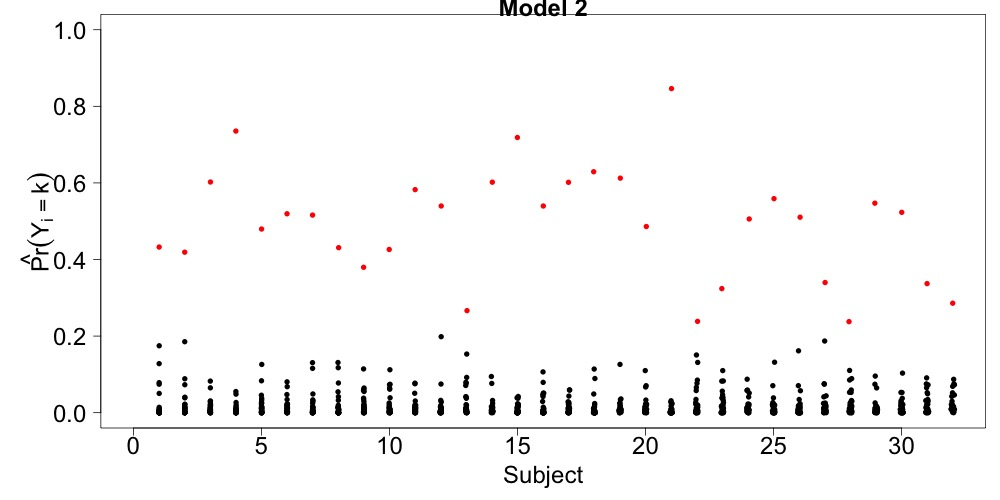
\includegraphics[width=\textwidth]{pred_subjs.jpeg}
\end{frame}



\begin{frame}
\frametitle{Predicting Subjects: Results}
\begin{itemize}
\item 75\% classification accuracy with Model 1
\end{itemize}
\centering
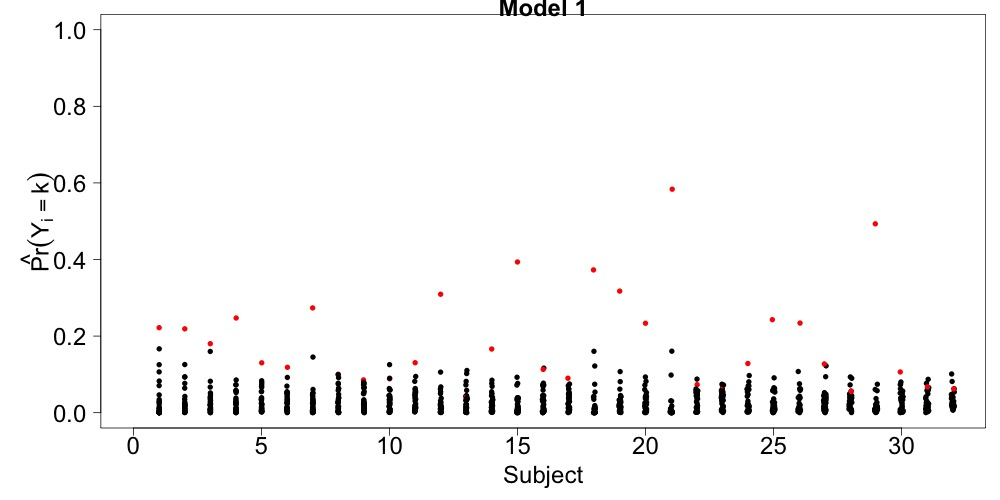
\includegraphics[width=\textwidth]{pred_subjs_m1.jpeg}
\end{frame}

\begin{frame}
\frametitle{Predicting Subjects: Training Data}
\centering
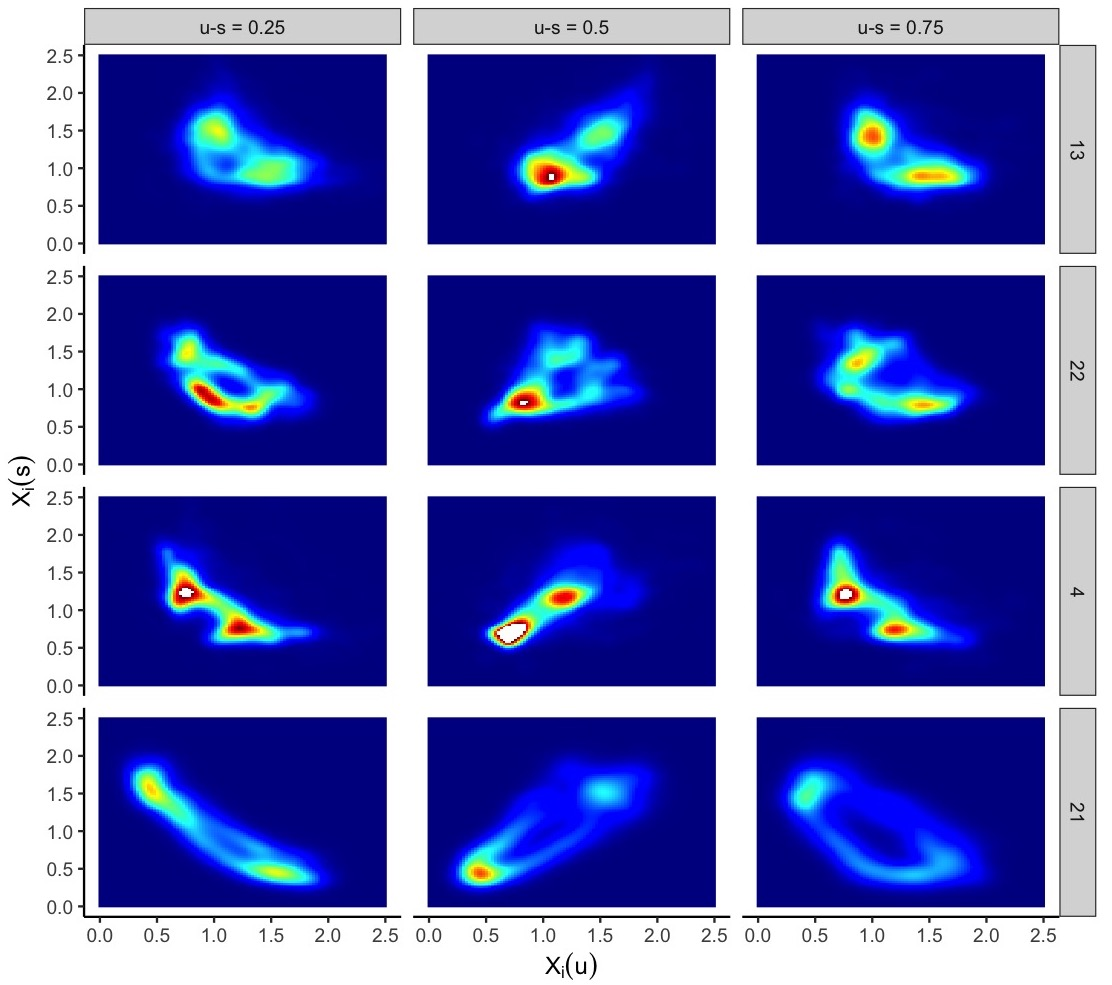
\includegraphics[height=\textheight]{kde_2d_fits_train.jpeg}
\end{frame}

\begin{frame}
\frametitle{Predicting Subjects: Test Data}
\centering
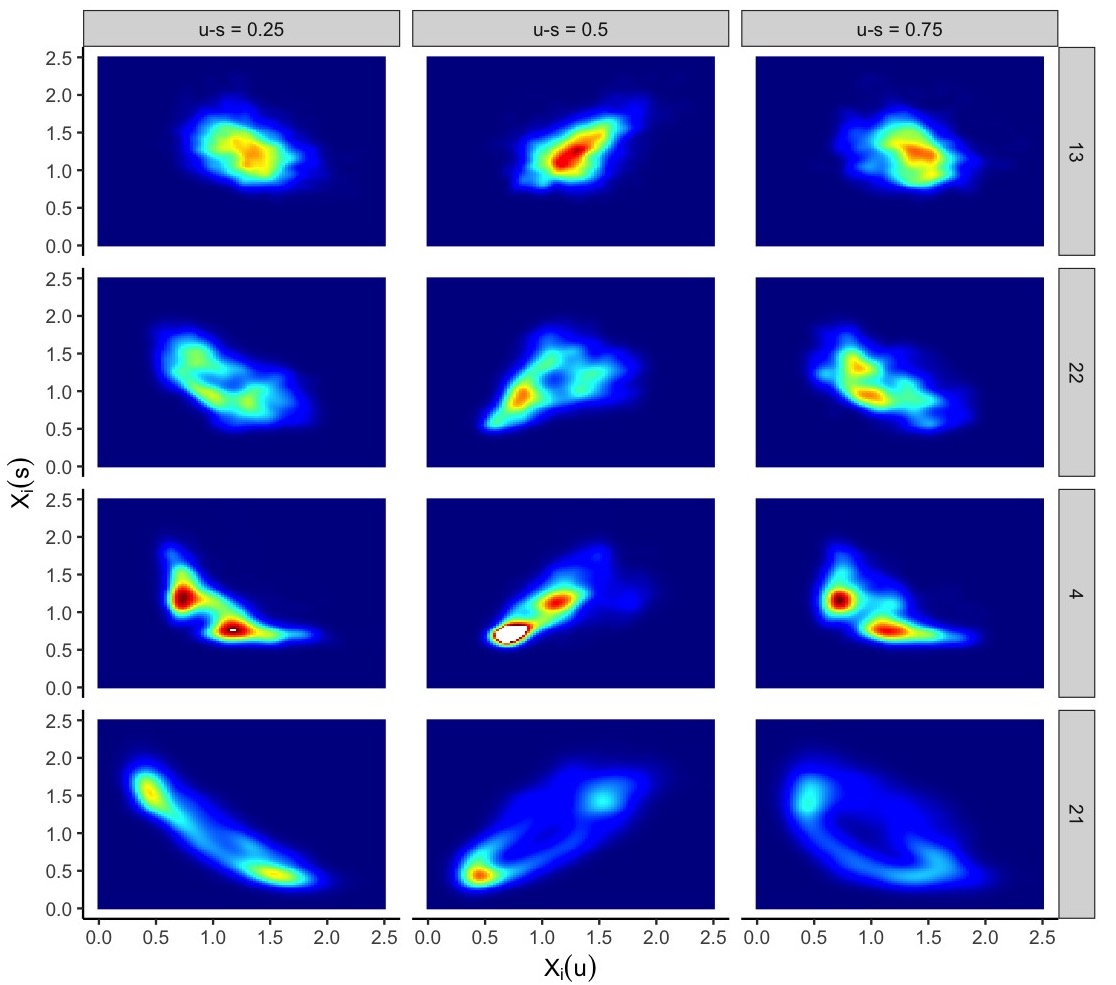
\includegraphics[height=\textheight]{kde_2d_fits_test.jpeg}
\end{frame}


% 
% \begin{frame}
% \frametitle{Predicting Subjects: Results}
% \begin{itemize}
% \item 100\% classification accuracy
% \end{itemize}
% \end{frame}
% 



\section{Concluding Remarks}
\begin{frame}
\frametitle{Some Thoughts}
\begin{itemize}
\item Limitations
    \begin{itemize}
    \item Requires labelled training and test data
    \item Need to choose interval length (computational and sample size concerns)
    \item Requires a definined population for comparison
    \item Computationally not expected to scale well 
    \item Lab walking vs ``in-the-wild" walking
    \end{itemize}
\item Proof of concept! Extracting patterns seems to hold some signal
\item Alternatives to functional regression
    \begin{itemize}
    \item Estimate 3-d densities (or 2-d conditional on s-u), establish some sort of thresholding
    \item Machine learning on the pairwise difference vectors 
    \end{itemize}
\end{itemize}
\end{frame}









\end{document}


